

\documentclass{beamer}
\usepackage{graphicx}
	\usetheme{Rochester}

\begin{document}
\title{University of Dodoma\\ 
College of Informatics and Virtual Education\\
School of Informatics\\

\includegraphics[scale=0.5]{udomlogo}
}
\author{Mnyawami Yuda\\
HD/UDOM/127/T.2014\\
\textbf{MSc Information Technology}\\
\textbf{Name of Lecturer:} Mr. Faustine Antony
} 
\date{\today} 

\begin{frame}
\titlepage
\end{frame}
\section{Introduction}
\begin{frame}
\frametitle{Outline:}
\begin{itemize}
\item What is 5G?\\
\item Drivers, goals, and challenges of 5G\\
\item Enabling technologies\\
\item CR in 5G\\
\item Broadening the CR concept\\
\item Dynamic Spectrum Access\\
\item Challenges on CR Implementation\\
\item Future Research Directions\\
\item Conclusion\\
\end{itemize}
 

\end{frame}
\section{What drives 5G?}
\begin{frame}
\frametitle{What drives 5G?}


\textbf{Mobile data demand will continue to increase.}\\

Growth of existing applications.\\
\begin{itemize}
\item e-mail,\\ 
\item file transfer,\\ 
\item real-time audio (VoIP),\\ 
\item Video streaming,\\
\item IP traffic,\\ 
\end{itemize}
\end{frame}

\begin{frame}
\frametitle{What drives 5G?}


\textbf{New applications and new ways of doing things
.}\\

\begin{itemize}
\item Instant Messaging (IM) with big files: lots of short connections, high data rates.\\
\item Internet-of-Things (IoT) and Machine-to-Machine (M2M): massive numbers of devices and connections, little data more than 50 billions of connected devices in 2020.\\
\item Critical applications - e.g., health, safety and security, traffic systems: guaranteed QoS.

\end{itemize}
\end{frame}

\begin{frame}
\frametitle{Cisco’s traffic prediction}
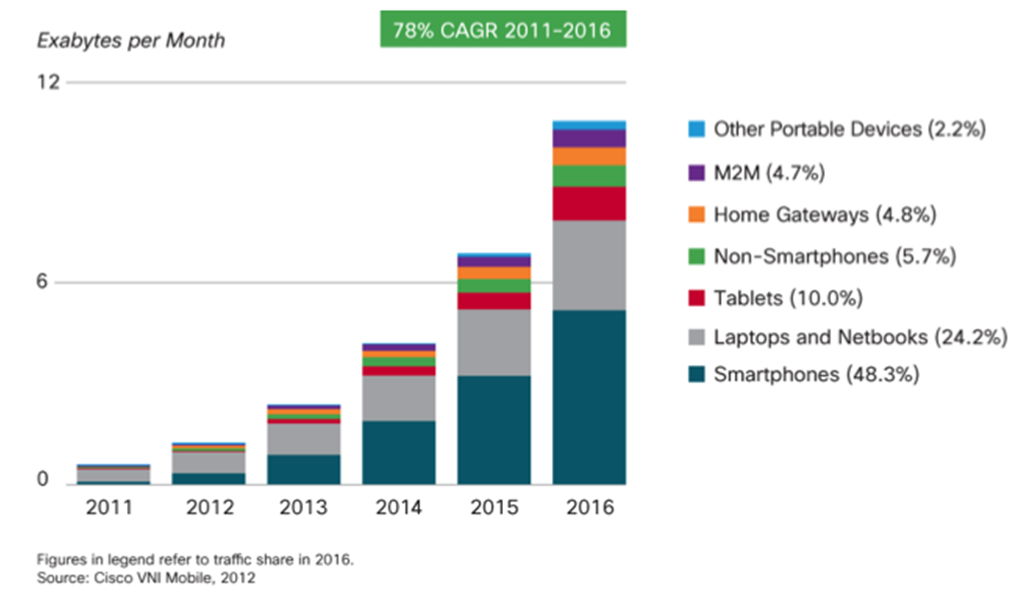
\includegraphics[scale=0.5]{cisco}
\end{frame}


\section{Multiple challenges}
\begin{frame}
\frametitle{Multiple challenges}
\textbf{Exploding traffic volume}
\begin{itemize}
\item Mobile data traffic growth more than 24-fold between 2010 and 2015, more than 500-fold between 2010 and 2020.
\end{itemize}
\textbf{Random and diverse traffic}
\begin{itemize}
\item Uneven distribution of traffic across space and time\\
\item Peak-to-mean traffic in fixed Internet up to 100:1; greater ratios expected for mobile broadband\\
\item Diversity of applications with very different QoS requirements\\
\end{itemize}
\textbf{Control plane load (IoT, IoE)}\\
\textbf{Low cost}\\
\textbf{Energy efficiency}\\

\end{frame}
\section{Goals}
\begin{frame}
\frametitle{Goals in 5G}
\begin{itemize}
\item Data Rates
\item Capacity
\item Spectrum
\item Energy
\item Latency
\item Reliability
\item Coverage
\item Devices per area
\end{itemize}
\end{frame}
\section{5G TECHNOLOGIES}
\subsection{Dense Heterogeneous Networks (HetNets)}
\begin{frame}
\frametitle{5G TECHNOLOGIES}
\textbf{Dense Heterogeneous Networks (HetNets)}
\begin{itemize}
\item \textbf{Macro cells combined with Small cells}: picocells and femtocells
	Increase of spectral efficiency, improved coverage, reduction of transmit power.
\item \textbf{Separation of data and control planes}
	Connectivity with two BS: macro for control, small cell for transport
\item \textbf{Multiple radio-access technologies}
	Including unlicensed and licensed shared access
\item \textbf{Device-to-device communication (D2D)}
	Increase energy efficiency, decrease interference, increase coverage

\end{itemize}
\end{frame}

\subsection{Self-Organizing Networks (SONs)}
\begin{frame}
\frametitle{5G TECHNOLOGIES}
\textbf{Self-Organizing Networks (SONs)}
\begin{itemize}
\item Self-configuration: neighbor discovery , coordinated selection of parameters, e.g., cell identity, Tx-power, time-frequency resource sharing
\item Saving of OPEX by reducing human interventions
\item SON needed for small cells where the number of deployed nodes could be very high

\end{itemize}
\end{frame}

\subsection{Software Defined (Cellular) Networks}
\begin{frame}
\frametitle{5G TECHNOLOGIES}
\textbf{Software Defined (Cellular) Networks}
\begin{itemize}
\item Directly programmable architecture
\item Simplified network management and control
\item Simplified introduction of new services or configuration changes
\item Fine-grained resource control

\end{itemize}
\end{frame}

\subsection{Indoor positioning}
\begin{frame}
\frametitle{5G TECHNOLOGIES}
\textbf{Indoor positioning}
\begin{itemize}
\item Additional information can help in resource allocation, and service improvement
\item Enabler of new applications
\end{itemize}
\end{frame}

\subsection{Intelligent user-device assistance}
\begin{frame}
\frametitle{5G TECHNOLOGIES}
\textbf{Intelligent user-device assistance}
\begin{itemize}
\item Sensing, relaying.
\item Machine learning.
\item Intelligent Transport System paradigm.

\end{itemize}
\end{frame}
\begin{frame}
\textbf{COGNITIVE RADIO IN 5G}
\end{frame}

\section{CR in 5G}
\begin{frame}
\frametitle{What will be the role of CR in 5G?}
\begin{itemize}
\item Will CR in 5G be a key technology or a nice-to-have feature?
\item Wouldn’t 5G loose its edge if CR spectrum access became dynamic and without guarantees?
\item Do we need to extend the concept of CR beyond spectrum?
\end{itemize}
\end{frame}

\subsection{Meaning}
\begin{frame}
\frametitle{Meaning of Cognitive Radio}

It is an intelligent wireless communication system that is aware of its surrounding environment (i.e., outside world), and uses the methodology of understanding by building to learn from the environment and adapt its internal states to statistical variations in the incoming RF stimuli by making corresponding changes in certain operating parameters (e.g., transmit power, carrier frequency and modulation strategy) in real-time, with two primary objectives in mind: highly reliable communications whenever and wherever needed; and efficient utilization of the radio spectrum”.

\end{frame}

\subsection{Motivation}
\begin{frame}
\frametitle{The Motivation behind Cognitive Radio}
\textbf{Significant underutilization of the radio spectrum.}\\
\textbf{The Cognitive Radio solution to the spectrum underutilization problem:}
\begin{itemize}

\item Sense the radio environment to detect spectrum holes (i.e., underutilized subbands of the radio spectrum).
\item Make the spectrum holes available for employment by secondary users efficiently, subject to the constraint that the received power in each spectrum hole does not exceed a prescribed limit (set by the legacy user).

\end{itemize}
\end{frame}

\subsection{How it works}
\begin{frame}
\frametitle{How it works}
\textbf{The cognitive radio network is a complex multiuser wireless communication system capable of emergent behaviour.}\\
\textbf{It embodies the following functions:}
\begin{itemize}
\item To perceive the radio environment (i.e., outside world) by empowering each user’s receiver to sense the environment on a continuous-time basis;
\item To learn from the environment and adapt the performance of each transceiver (transmitter-receiver) to statistical variations in the incoming RF stimuli;
\end{itemize}
\end{frame}



\subsection{How it works}
\begin{frame}
\frametitle{How it works cont..}
\begin{itemize}
\item To facilitate communication between multiple users through cooperation in a self-organized manner;
\item To control the communication processes among competing users through the proper allocation of available resources;
\item To create the experience of intention and self-awareness.

\end{itemize}
\end{frame}

\subsection{Objectives}
\begin{frame}
\frametitle{Primary objectives}
\begin{itemize}
\item To provide highly reliable communication for all users of the network.
\item To facilitate efficient utilization of the radio spectrum in a fair-minded way.
\end{itemize}
\end{frame}

\subsection{Why may CR be interesting for 5G?}
\begin{frame}
\frametitle{Why may CR be interesting for 5G?}
\begin{itemize}
\item Some bands are significantly underutilized
\item Cost of dynamically leasing spectrum is expected to be much lower than purchasing a licensed band
\item Allows expansion of spectrum at a much lower cost
\item Coping with overload traffic
\end{itemize}
\end{frame}

\begin{frame}
\textbf{Challenge: How to use those complementary resources to optimize system performance?}
\end{frame}

\section{Architectures of Cognitive Cellular Networks}
\subsection{Non-Cooperative Architecture}
\begin{frame}
\frametitle{Non-Cooperative Architecture}
\begin{itemize}
\item Two separated networks at the physical layer
\item Integration at upper layers

\end{itemize}
\end{frame}

\section{Architectures of Cognitive Cellular Networks}
\subsection{Cooperative Architecture}
\begin{frame}
\frametitle{Cooperative Architecture}
\begin{itemize}
\item Combined used of licensed and CR resources to form a single integrated network
\item Using cooperative communication principles (coordinated relaying by users)
\item Major performance gains possible
\end{itemize}
\end{frame}

\begin{frame}
\frametitle{Non-Cooperative Architecture}
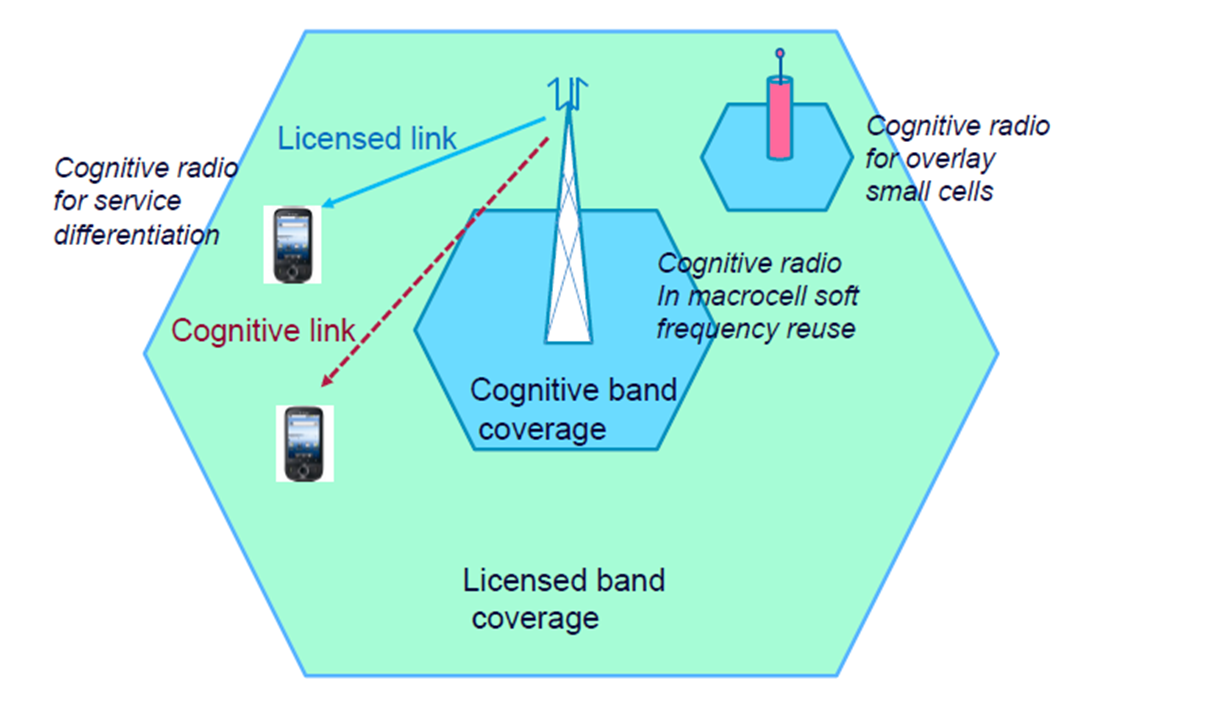
\includegraphics[scale=0.5]{nonartch}
\end{frame}


\begin{frame}
\frametitle{Usage scenarios}
\begin{itemize}
\item Power-limited cognitive radio resources for users near the macro-cell; licensed resources for users far away.
\item Service differentiation: licensed resources for strict QoS demands and CR for relaxed QoS
\item Cognitive small cells (femtocells) using CR to cover traffic hot spots or coverage gaps.
\end{itemize}
\end{frame}

\begin{frame}
\frametitle{Cooperative Architecture}
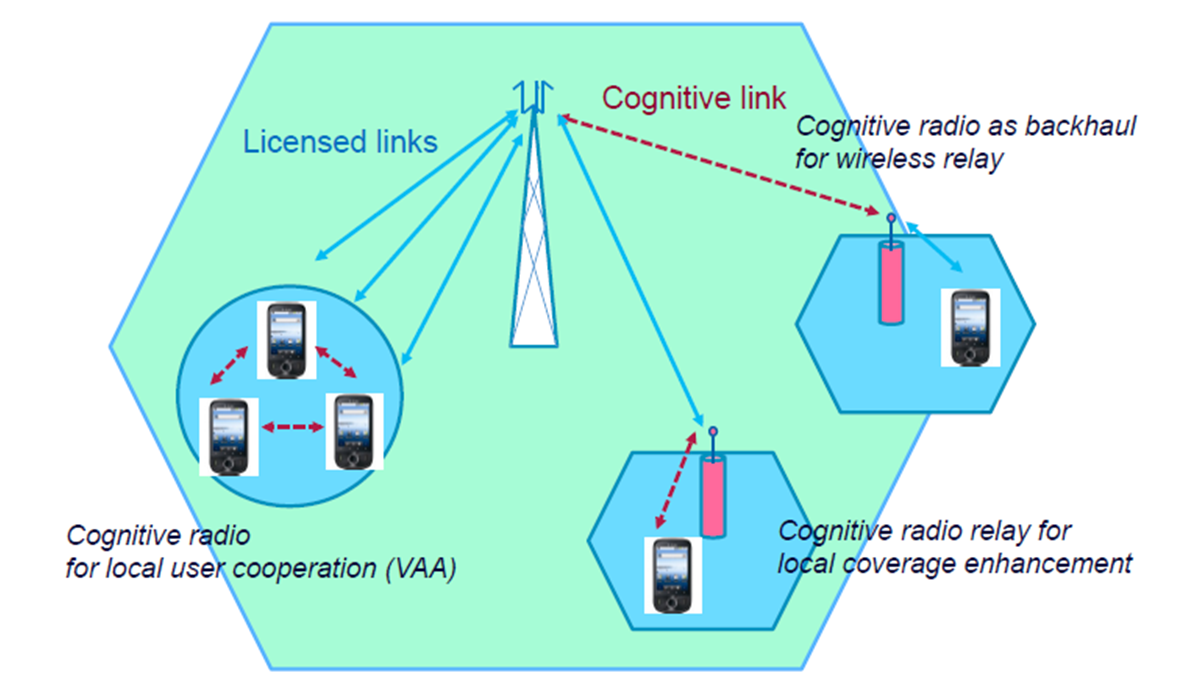
\includegraphics[scale=0.5]{arch}
\end{frame}


\begin{frame}
\frametitle{Usage scenarios}
\textbf{Cognitive relay for capacity enhancement}
\begin{itemize}
\item Communication to BS with licensed resources; CR for local coverage
\item Communication to BS with CR; local coverage with licensed resources: no modification for conventional user devices
\textbf{Virtual Antenna Array (VAA)}
\item Virtual MIMO in licensed band: performance gains
\end{itemize}
\end{frame}

\begin{frame}
\frametitle{Major Functional Blocks of Cognitive Radio}
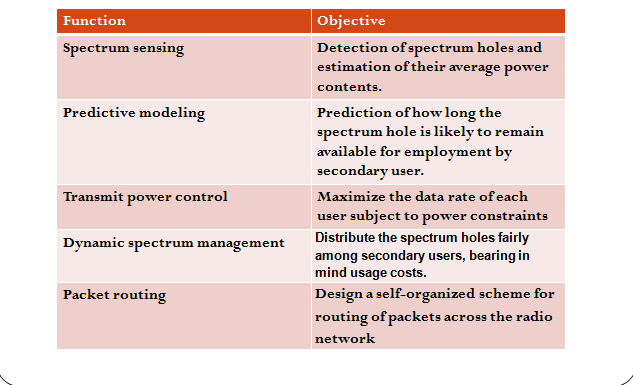
\includegraphics[scale=0.75]{fns}
\end{frame}

\section{Main in CR issues}
\begin{frame}
\frametitle{Main in CR issues}
\textbf{Self Coexistence}\\
\begin{itemize}
\item To avoid secondary users to harmfully interfere with primary users.\\ 
\end{itemize}
\textbf{Accurate sensing}\\
\begin{itemize}
\item Sensing aims to determine if a channel is idle or busy in terms of primary user activity.\\
 \end{itemize}
\textbf{Optimized spectrum decision}\\
\begin{itemize}
\item Secondary users are expected to dynamically choose the best available channels and transmission parameters.\\
\end{itemize} 
\textbf{Seamless spectrum handover}\\
\begin{itemize}
\item No latency should be noticed by users during mobility.
\end{itemize} 
\end{frame}

\section{Main in CR issues}
\begin{frame}
\frametitle{Main in CR issues cont..}
\textbf{Cross layer design}\\
\begin{itemize}
\item Spectrum sensing is restricted only to the PHY and MAC layers, spectrum management (e.g., spectrum handover, decision making and scheduling) can be related to all upper layers, which makes interaction and coordination between the different layers of the protocol stack necessary.\\ 
\end{itemize}
\textbf{Energy efficiency}\\
\begin{itemize}
\item Have limited communication and resource requirements, since most of the devices are battery powered. 
\end{itemize}


\end{frame}

\section{Standards}
\begin{frame}
\frametitle{Standards}
\textbf{The IEEE 802.22 }
\begin{itemize}
\item It is the first effort for achieving a CR international standard.
\item It defines CR techniques that are specifically targeted to enable unlicensed devices to exploit television white spaces in the VHF and UHF bands (54-862 MHz) in a non-interfering basis for the deployment of Wireless Regional Area Networks (WRAN). 
\end{itemize}

\end{frame}

\section{Standards}
\begin{frame}
\frametitle{Standards}
\textbf{The IEEE SCC41 (Standards Coordinating Committee 41)}
\begin{itemize}
\item Formerly known as IEEE P1900, addresses the area of Dynamic Spectrum Access Networks (DySPAN) and aims to develop standards for next generation radio and advanced spectrum management. 
\end{itemize}
\end{frame}


\section{LEARNING BASED ON PAST EXPERIENCE}
\begin{frame}
\frametitle{Learning}
\textbf{Spectrum decision can be performed reactively, as a consequence of an unexpected link failure, or proactively through anticipation.}\\

\textbf{Benefits of proactive spectrum decision are: }\\
\begin{itemize}
\item Decrease of time and energy spent to find an idle channel before any transmission, as channels can be prioritized according to their probabilities of availability 
\end{itemize}
\end{frame}

\begin{frame}
\frametitle{Learning cont..}
\begin{itemize}
\item Decrease in the number of spectrum handovers and service interruption losses, because channels can be prioritized according to their expected durations of availability
\item Decrease in terms of interference to primary users, as primary user appearance can be probabilistically determined during transmission.
\end{itemize}
\end{frame}

\section{Dynamic Spectrum Access (DSA)}
\begin{frame}
\frametitle{Dynamic Spectrum Access}

\textbf{It refers to the method used to detect and to access spectrum holes.}\\
This term is very broad and contains a number of elements like:
\begin{itemize}
\item spectrum access
\item spectrum allocation
\item spectrum pooling
\item spectrum management
\item regulation activities
\end{itemize}
\end{frame}
\begin{frame}
\frametitle{Dynamic Spectrum Access\dots}
\begin{itemize}
\item The spectrum is allocated opportunistically and the goal is to achieve device-centric interference control and dynamic reuse of the spectrum.

\end{itemize}
\end{frame}

\begin{frame}
\frametitle{Dynamic Spectrum Access\dots}
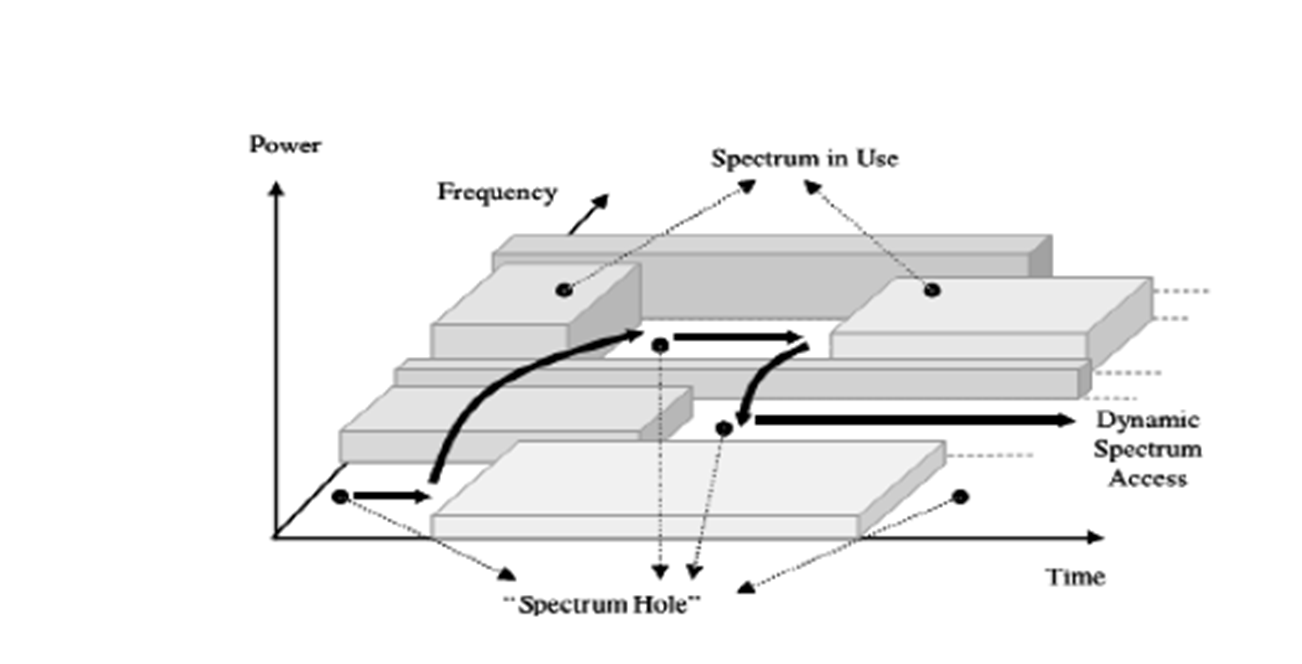
\includegraphics[scale=0.5]{dsa}

\end{frame}



\subsection{Models of DSA}
\begin{frame}
\frametitle{Categories of DSA}
\textbf{There are three general categories of DSA}
\begin{itemize}
\item Between a licensed primary system and a license-free secondary system, e.g., used to access the digital TV spectrum.
\item Within the same primary system (to share the 3G/4G spectrum), with the help of, e.g., femtocells.
\item Between two primary systems used at spectrum trading among cellular operators.
\end{itemize}

\end{frame}
\begin{frame}
\frametitle{Models of Dynamic Spectrum Access}
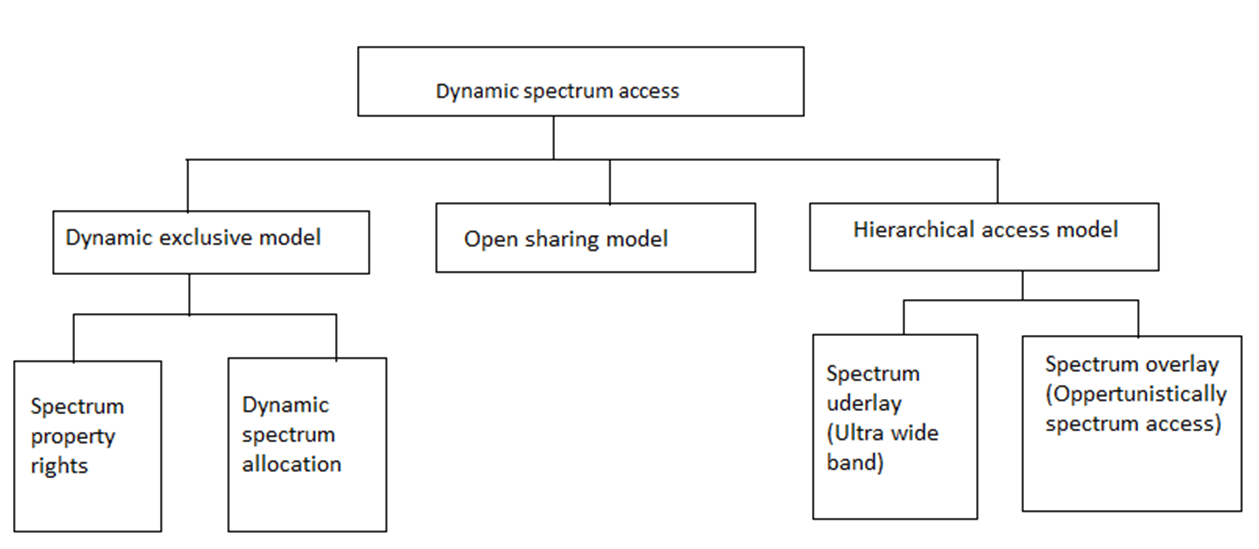
\includegraphics[scale=0.5]{models}
\end{frame}

\subsubsection{Dynamic exclusive use model}
\begin{frame}
\frametitle{Dynamic exclusive use model}
\begin{itemize}
\item It maintains the basic structure of the existing policy for spectrum regulation.\\
\item The spectrum is allocated to certain services for exclusive use, at particular times and in particular geographic regions. This approach cannot eliminate the white space in spectrum, which may result from the busty nature of the wireless traffic.
\end{itemize}

\end{frame}

\begin{frame}
\frametitle{Open sharing model}
\begin{itemize}
\item It is used by competing peer users to share the available spectrum in a spectral region. 
\item Different spectrum sharing strategies can be used in this case, e.g., centralized, distributed. 
\item This model is popular in diverse wireless services operating in industrial, scientific and medical environments.

\end{itemize}

\end{frame}

\subsubsection{Open sharing model}
\begin{frame}
\frametitle{Open sharing model}

\textbf{Uncontrolled-commons}
\begin{itemize}
\item This is also referred as open spectrum access. When a spectrum band is managed no entity has exclusive licensed to the spectrum band. It is maximum transmit power constraint.
\end{itemize}
\textbf{Managed-commons}
\begin{itemize}
\item This represents an effort to avoid the tragedy of commons by imposing a limited form of order or structure of spectrum access.
\end{itemize}
\textbf{Private-commons}
\begin{itemize}
\item Spectrum owner specifies technology and protocol for the CR user access.
CR user may receive a command from spectrum owner (transmission parameter). CR user may sense and access the spectrum.
\end{itemize}

\end{frame}

\subsubsection{Hierarchical access model}
\begin{frame}
\frametitle{Hierarchical access model}
\textbf{Hierarchical access model}
\begin{itemize}
\item It is used to the primary and secondary users. 
\item The basic idea is to open the licensed spectrum to secondary users provided that the interference perceived by the primary (licensees) users is limited.
\end{itemize}

\textbf{There are also two types of model}
\begin{itemize}
\item Spectrum overlay
        -High noise of Secondary User against Primary User
\item Spectrum underlay
		-Low noise of Secondary User against Primary User
\end{itemize}

\end{frame}

\begin{frame}
\frametitle{ Hierarchical access model}

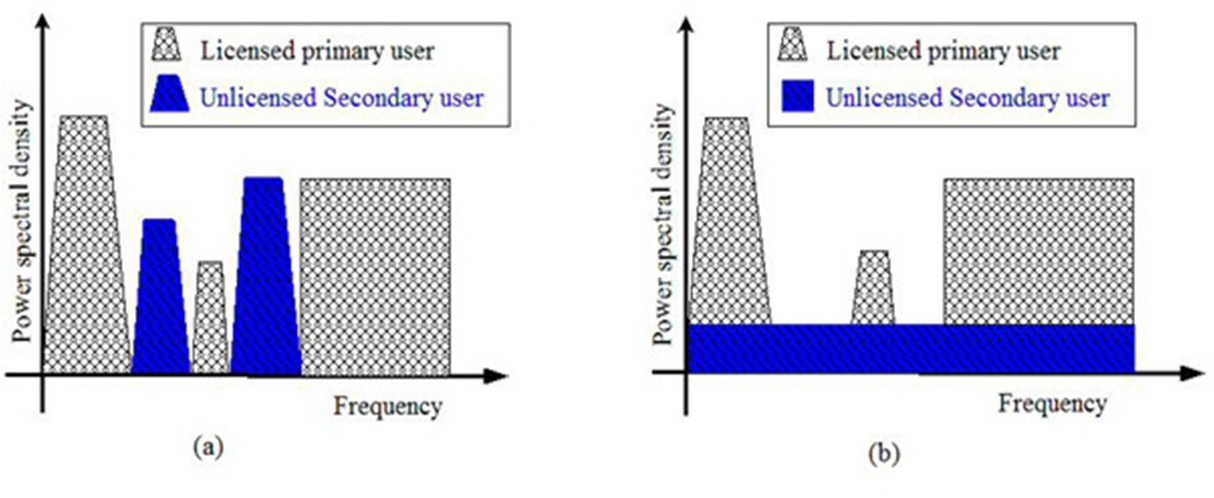
\includegraphics[scale=0.5]{hiera}

\end{frame}

\section{Implementation Challenges}
\begin{frame}
\frametitle{Implementation Challenges}
\begin{itemize}
\item RF Front-Ends Transceiver Challenges.
\item ADC and DAC Challenges.
\item Baseband Challenges.
\item Spectrum Sensing Algorithm Implementation.
\end{itemize}
\end{frame}

\section{Future Research Directions}
\begin{frame}
\frametitle{Implementation Challenges}
\begin{itemize}
\item Seamless spectrum handovers
\item Proactive spectrum selection and interference avoidance
\item Interdependency between the propagation characteristics of radio signals and the frequency band in usage Energy efficiency
\item Validation of CR protocols\\
GNU Radio/USRP-based.\\
ORBIT (Open Access Research Testbed for Next-Generation Wireless Networks).
\item Security 

\end{itemize}
\end{frame}

\section{Conclusion}
\begin{frame}
\frametitle{Conclusion}
\begin{itemize}
\item CRS offers also the possibility of flexibly managing the spectrum in a dynamic manner in heterogeneous radio access networks. 
\item Through intelligent management mechanisms, frequency bands can be allocated to Radio Access Technologies(RATs) dynamically in a way such that the capacity of each RAT is maximized and interference is minimized
\item Network operator may employ different RATs dynamically over time/frequency/location and acquire or exchange the spectrum usage rights. 
\item The cognitive devices may autonomously and dynamically adapt to the diverse heterogeneous radio access networks.
\item CR area, which is still in its infancy and aims to enable an efficient utilization of the radio spectrum.

\end{itemize}
\end{frame}

\end{document}

